\chapter*{Instalação e configuração do ambiente}
\label{apendice:1}

\section*{Controlador de versão}

Nesta seção serão apresentado os passos necessários para a criação do repositório utilizado no sistema de controle de versão, junto com a instalação da ferramenta utilizada para trabalhar com este controlador de versão e sua configuração.

Para criar um repositório no Github (ferramenta de controle de versão) utilizado neste trabalho, deve-se acessar a  \textit{url} http://github.com, por meio de um navegador de internet e clicar no botão \textit{"Sign In"}, caso possua conta, caso contrário clique no botão \textit{"Sign up"} e crie sua conta. A Figura~\ref{fig:ap1:pagina_inicial_github} apresenta a página inicial do Github.

\captionsetup[figure]{list=no}
\begin{figure}[h!]
	\centerline{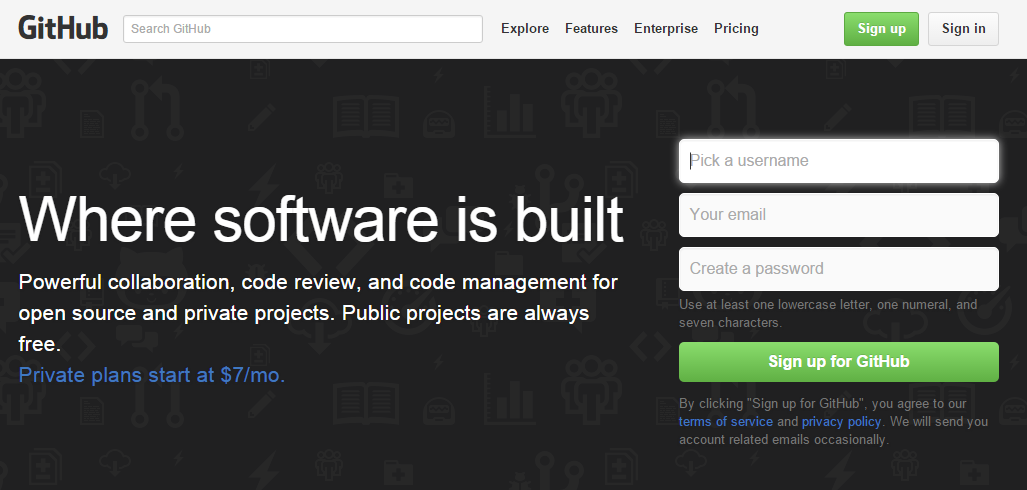
\includegraphics[scale=0.55]{./imagens/apendices/pagina-inicial-github.png}}
	\caption[Página inicial do Github.]
	{Página inicial do Github. \textbf{Fonte:} Elaborado pelos autores.}
	\label{fig:ap1:pagina_inicial_github}
\end{figure}

Para prosseguir no processo de criação do repositório (com a conta já criada), basta clicar no menu \textit{"Sign In"}, realizar o \textit{login} e a página inicial, contendo a lista de seus repositórios será apresentada conforme a Figura~\ref{fig:ap1:pagina_home_github} apresenta.

\newpage
\captionsetup[figure]{list=no}
\begin{figure}[h!]
	\centerline{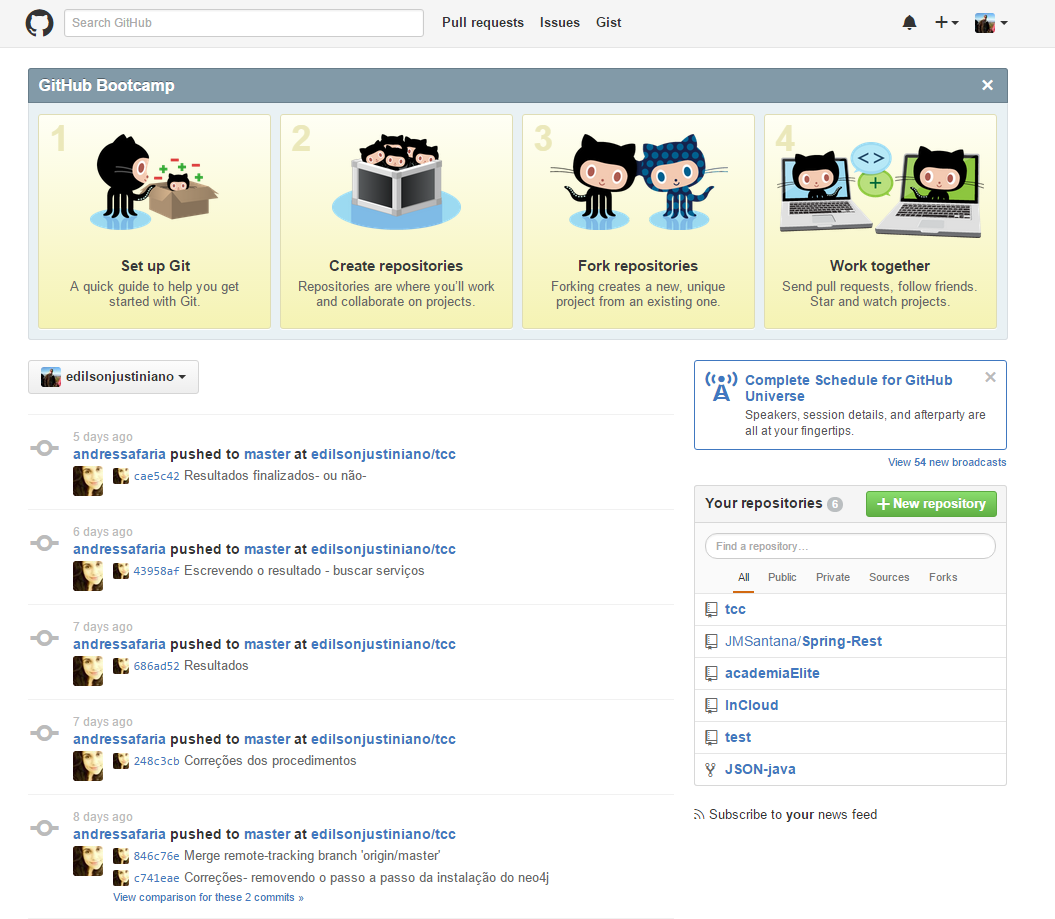
\includegraphics[scale=0.55]{./imagens/apendices/pagina-home-github.png}}
	\caption[Página com a lista de repositórios do usuário no Github.]
	{Página com a lista de repositórios do usuário no Github. \textbf{Fonte:} Elaborado pelos autores.}
	\label{fig:ap1:pagina_home_github}
\end{figure}

 
Nesta seção serão apresentados os passos para a instalação do banco de dados Neo4j.